%\documentclass[pageno]{jpaper}
\documentclass[twocolumn]{article}

\usepackage{latexsym}
\usepackage{amssymb}
\usepackage{amsmath}
\usepackage{graphicx}
\usepackage{cite}
\usepackage{alltt}
\usepackage{url}
\usepackage{xspace}
\usepackage{extarrows}
\usepackage{soul}
\usepackage{multirow}
\usepackage{listings}
\setstcolor{red}
\usepackage[utf8]{inputenc}
\usepackage[T1]{fontenc}
\usepackage[normalem]{ulem}
\usepackage{comment}
\usepackage{times}

\pagestyle{empty}
%set paper size
%for A4 paper
\topmargin      29mm    %bottom margin 30mm
\oddsidemargin  15mm    %left & right margin 15mm

%for 8 1/2" x 11" paper paper, use the following definition
%\topmargin     17mm    %bottom margin 24mm
%\oddsidemargin 18mm    %left margin 18mm & right margin 17mm

%text sizes
\textwidth  180mm
\textheight 238mm
\columnsep  5.0mm
\parindent  3.5mm

%misc parameters
\headsep 0mm  \headheight 0mm
\footskip 18mm
%\footheight 6mm

%conversion to values for LaTeX
\advance\topmargin-1in\advance\oddsidemargin-1in
\evensidemargin\oddsidemargin

\makeatletter
%as Latex considers descenders in its calculation of interline spacing,
%to get 12 point spacing for normalsize text, must set it to 10 points
\def\@normalsize{\@setsize\normalsize{12pt}\xpt\@xpt
\abovedisplayskip 10pt plus2pt minus5pt\belowdisplayskip \abovedisplayskip
\abovedisplayshortskip \z@ plus3pt\belowdisplayshortskip 6pt plus3pt
minus3pt\let\@listi\@listI}

%interline spaceing and title font for section
\def\section{\@startsection {section}{1}{\z@}{20pt plus 2pt minus 2pt}
{8pt plus 2pt minus 2pt}{\centering\normalsize\sc
\edef\@svsec{\thesection.\ }}}
\def\thesection{\Roman{section}}

%interline spacing and title font for subsection
\def\subsection{\@startsection {subsection}{2}{\z@}{16pt plus 2pt minus 2pt}
{6pt plus 2pt minus 2pt}{\normalsize\sl
\edef\@svsec{\thesubsection.\ }}}
\def\thesubsection{\Alph{subsection}}

%figures/tables captions
\long\def\@makecaption#1#2{
\vskip10pt\begin{center} #1 #2 \end{center}\par\vskip 1pt}
\def\fnum@figure{\raggedright{\footnotesize Fig. \thefigure }.%
\footnotesize}
\def\fnum@table{\footnotesize TABLE \thetable\\\footnotesize\sc}
\def\thetable{\Roman{table}}

\makeatother

%%%%%%%%%%%%%%%%%%%%%%%%%%%%%%%%%%%%%%%%%%%%%%%%%%%%%%%%%%%%%%%%%%%%%%%

\newcommand{\hcinv}{\texttt{hc\_inversion}\xspace}
\newcommand{\coqdockw}[1]{\texttt{#1}}
\newcommand{\inversion}{\coqdockw{inversion}\xspace}
\newcommand{\inv}{\coqdockw{inv}\xspace}
\newcommand{\simlight}{\texttt{Simlight}\xspace}
\newcommand{\compcert}{\texttt{CompCert}\xspace}
\newcommand{\clight}{\texttt{Clight}\xspace}
\newcommand{\simsoc}{\texttt{SimSoC}\xspace}
\newcommand{\simsoccert}{\texttt{SimSoC-Cert}\xspace}
\newcommand{\stt}{\small\tt}
\newcommand{\why}{\texttt{Why}\xspace}
\newcommand{\whyML}{\texttt{WhyML}\xspace}
\newcommand{\whyCert}{\texttt{WhyCert}\xspace}
\newcommand{\framac}{\texttt{Frama-C}\xspace}


%replace XXX with the submission number you are given from the ASPLOS submission site.
% \newcommand{\asplossubmissionnumber}{XXX}

\begin{document}
%date not printed
\date{}

%make title
\title{\Large\bf
Certified Simulation: What You Get Is What You Want}
\author{Authors omitted for review\\room for authors addresses\\}
\maketitle
\thispagestyle{empty}

{\small\bf Abstract---
  This paper presents an approach for certified virtual prototyping of
  embedded software. The machine code executed on a target
  architecture can be proven to provide the same results as the
  initial algorithm, and the proof is verified with an automated
  theorem prover. This requires the establishment of a tool chain in
  where each step can be certified. The paper presents the proof of an
  ARM architecture Instruction Set Simulator all of the proofs being
  verified with the Coq theorem prover.}

\section{Introduction}

In many applications, it is desirable to exhibit a proof of program to
certify that the execution of a given algorithm is correct on the
specific computer architecture on which the program is executed. For
example in the area of cryptography it is interesting to be certain
that the resulting encrypted data output by the computer is indeed the
same as the result obtained with the formal method describing the
algorithm, coded through some programming language and compiled
into machine code.

Obtaining such certification is not a one step proof, it consists in a
series of steps requiring a tool chain. In this paper, we present an
attempt towards building such a certification chain, including a
certified simulator of processor architecture. Our approach towards
this certification of programs is the following: given the formal
specification of an algorithm, for example the DES cryptographic
encryption technique, one can derive a C program using formal methods
such as B \cite{abrial-1996} or SCR \cite{rothamel-2006} or APTS
\cite{apts-2008}.  In this paper we assume that this phase has been
achieved, that there is an existing C source code program that is a
provably correct implementation of the specification. Our purpose is
to show how it can be certified that the execution of that C program
on the instruction set simulator of a target architecture indeed
produces the expected results.  This requires sequential steps, to
prove first that the translation from C code to machine code is
correct, and second that the simulation of the machine code is also
correct, that is, they preserve the semantics of the source code;
together with the fact that all of these proofs are verified using a
theorem prover or proof checker, not subject to human error in the
proof elaboration or verification.

The technique presented here relies on already existing tools,
in particular the Coq proof assistant, the Compcert C compiler, a
certified compiler for the C language, combined with our own work to
prove the correctness of an ARM Instruction Set Simulator, integrated
within an existing virtual prototyping framework.

The sequel of the paper presents the background existing tools,
related work, our method to combine these tools and our additional work
to reach the objectives.


%%%%%%%%%%%%%%%%%%%%%%%%%%%%%%%%%%%%%%%%%%%%%%%%%%%%%%%%%%%%%%%%%%%%%%%%%%%%%
\section{Related Work}
\label{related}

Program certification has to be based on a formal model of the program
under study.  Such a formal model is itself derived from a formal
semantics of the programming language.  Formal semantics are important
because they provide an abstract, mathematical, and standard
interpretation of a programming language.  There are three traditional
ways to express how programs perform computations: axiomatic
semantics, denotational semantics, and operational semantics.  An
overview of programming language semantics can be found in
\cite{nielson1992semantics, gunter-1992, winskel-1993}.

Denotational semantics \cite{stoy-denotational} constructs
mathematical objects which describe the meaning of expressions of the
language using stateless partial \emph{functions}.  All observably
distinct programs have distinct denotations.

Axiomatic semantics and Hoare logic\cite{Floyd67, Hoare-1969} have
been widely used for proving the correctness of programs.  For
imperative programming languages such as C, a possible approach is to
consider tools based on axiomatic semantics, like
\framac~\cite{canet2009value}, a framework for a set of interoperable
program analyzers for C. Most of the modules integrated inside rely on
ACSL (ANSI/ISO C Specification Language), a specification language
based on an axiomatic semantics for C.  ACSL is powerful enough to
express axiomatizations directly at the level of the C program.  State
labels can be defined to denote a program control point, and can then
be used in logic functions and predicates.

\framac software leverages off from \why technology
\cite{bobot2011why3, filliatre07cav}, a platform for deductive program
verification, which is an implementation of Dijkstra's calculus of
weakest preconditions.  \why compiles annotated C code into an
intermediate language.  The result is given as input to the VC
(Verification Conditions) generator, which produces formulas to be
sent to both automatic provers or interactive provers like Coq.

Paolo Herms's \cite{herms13phd}~\cite{herms2012certified} has provided
a certified verification condition generator for several provers,
called \whyCert.  This VC generator was implemented and proved sound
in Coq.  To make it usable with arbitrary theorem provers as
back-ends, it is generic with respect to a logical context, containing
arbitrary abstract data types and axiomatisations.

In our case of verifying an instruction set, as we need to deal both
with a very large specification including complex features of the C
language, we needed a framework that is rich enough to make the
specification manageable, using abstraction mechanisms for instance,
in which an accurate definition of C features is available.
Automated computations of weakest preconditions
and range of variation are not relevant in our case.
We need to verify more specific properties referring
to a formal version of the ARM rchitecture.
It was unclear that \framac would satisfy those requirements,
even with Coq as a back-end.

Operational semantics is a more concrete approach to program semantics
as it is based on states, although in contrast with a low-level
implementation, operational semantics considers abstract states.  The
behavior of a piece of program corresponds to a transition between
abstract states.  This transition relation makes it possible to define
the execution of programs by a mathematical computation \emph{relation}.
This approach is quite convenient for proving the
correctness of compilers, using operational semantics for the source
and target languages (and, possibly intermediate languages).

Operational semantics can be presented in two styles.  Small-step
semantics, often known as structural operational semantics, is used to
describe how the single steps of computations evaluate.  The other is
big-step semantics, or natural semantics, which returns the final
results of an execution in one big step.  The corresponding transition
relation is defined by rules, according to the syntactic constructs of
the language, in a style which is inspired by natural deduction. The
book \cite{nielson1992semantics} discusses the choices between
small-step semantics and big-step semantics depending on the
objective.  They sometimes can be equivalent.  But in general, they
provide different views of the same language and one has to choose an
appropriate one for a particular usage.  Moreover, some language
constructs can be hard or even impossible to define with one of these
semantics whereas it may be easy with the other style.  In general,
when big-step semantics can be used, it is simpler to manage than
small-step semantics. A tutorial on programming language semantics
made by Benjamin C. Pierce's \cite{pierce-tut} is mainly dedicated to
operational semantics and the material presented in this tutorial is
formalized in the Coq proof assistant.

Operational semantics is used in \compcert to define the execution of
C programs, or more precisely programs in the subset of C considered
by the \compcert project.  The work presented in this paper is based
on this approach.  Interesting examples are given by Brian Campbell in
the CerCo project~\cite{campbell2012executable}, in order to show that
the evaluation order constraints in C are very lax and not uniform.

Regarding formalization and proofs related to instruction set, a Java
byte code verifier has been proved by Cornelia Pusch\cite{pusch-1999},
the Power architecture semantics has been formally specified in
\cite{alglave-2009}, and closer to our work, the computer science
laboratory in Cambridge University has used HOL4 to formalize the
instruction set architecture of ARM~\cite{FoxM10}. The
objective of this work was to verify an implementation of this
architecture with \emph{logical gates}, whereas for \simsoc, we
consider a ARM simulator coded in C.  Reusing the work done at Cambridge
was considered for our work.  However, as our approach is based on
\compcert, which is itself coded in Coq instead of HOL4, it was more
convenient to develop our formal model and our proofs in Coq.

%%%%%%%%%%%%%%%%%%%%%%%%%%%%%%%%%%%%%%%%%%%%%%%%%%%%%%%%%%%%%%%%%%%%%%%%%%%%%
\section{Background} %
\label{background}

\subsection{Coq}

Coq\cite{coqart} is an interactive theorem prover, implemented in
OCaml. It allows the expression of mathematical assertions,
mechanically checks proofs of these assertions, helps to discover
formal proofs, and extracts a certified program from the constructive
proof of its formal specification.  Coq can also be presented as a
dependently typed $\lambda$-calculus (or functional language).  For a
detailed presentation, the reader can consult \cite{coqmanual} or
\cite{coqart}.  Coq proofs are typed functions and checking the
correctness of a proof boils down to type-checking. For example, a
proof term of type $\forall~n: nat,~P\, n~\rightarrow Q\, n$ 
is a function $fun~(n:nat) (p:P\:n)$ which takes a
natural number $n$ and a proof $p$ of $P\:n$ as arguments and returns
a proof of $Q\:n$.

Coq is not an automated theorem prover: the logic supported by Coq
includes arithmetic; therefore it is too rich to be decidable.
However, type-checking (in particular, checking the correctness of a
proof) is decidable.  As full automation is not possible for finding
proofs, human interaction is essential.  The latter is realized by
\emph{scripts}, which are sequences of commands for building a proof
step by step.  Coq also provides built-in tactics implementing various
decision procedures for suitable fragments of the calculus of
inductive constructions and a language 
% called \texttt{Ltac} % unused in this paper
which can
be used for automating the search of proofs and shortening scripts.

An interactive proof assistant, such as Coq, requires man-machine
collaboration to develop a formal proof.  Human input is needed to
create appropriate auxiliary definitions, choose the right inductive
property and, more generally, to define the architecture of the proof.
Automation is used for non-creative proof steps and checking the
correctness of the resulting formal proof.  A rich logic can be
handled in an interactive proof assistant for a variety of problems.

On the other hand, fully automated theorem provers have been
developed.  They can perform the proof tasks automatically, that is,
without additional human input.  Automated theorem prover can be
efficient in some cases.  However being able to automatically prove a
formula means that the problems solved belongs to a decidable, or at
least semi-decidable, class. Decidable logic are less powerful
expressive than higher-order logic, hence the range of
problems one can easily or at least conveniently model 
with an automated theorem prover is smaller
than with an interactive proof assistant.  In practice, both
approaches are important in the fields of computer science and
mathematical logic.  In our project, as a rich logical system is
needed in order to manage the complexity of the ARM specification and
of the proofs of C programs, we decided to use Coq.

\subsection{Compert-C}
\compcert is a formally verified compiler for the C programming
language provided by INRIA \cite{ccc, Leroy-Compcert-CACM}, which
currently targets Power, ARM and 32-bit x86 architectures.  The
compiler is specified, programmed, and proved in Coq. It aims to be
used for programming embedded systems requiring high reliability. The
performance of its generated code is often close to that of gcc
(version 3) at optimization level O1, and is always better than that
of gcc without optimizations.

It has a complex translation chain of eleven steps, from C source code
into assembly code. Every internal representation has its own syntax
and semantics defined in Coq. It is formally verified in the sense
that generated assembly code is proved to behave exactly the
same as the input C program, according to a formally defined
operational semantics of the language, and assumptions on the
instruction set.

Of course, if the input consists of C language expressions that are
ill-defined, according to the ISO-C specification, (i.e.  a[i++] = i;)
Compert-C generates ill-formed code. It generates verified code when
the input is what ISO-C defines as 'correct C program', which is expected
if the C code has been generated using formal specifications.

In our work, we use three parts of \compcert C.  The first is that we
use the correct machine code generated by the C compiler.  The second
is the C language operational semantics in Coq (its syntax and
semantics), from which we get a formal model of the program.  Third,
we use the \compcert basic library. It defines Coq data types for words,
half-words, bytes etc., and bitwise operations and lemmas to describe
their properties.  In our Coq model, we also use these low level
representations and operations to describe the instruction set model.

\subsection{SimSoC}

In this section, we introduce our certification target architecture,
based upon \simsoc~\cite{simsoc-llvm-2011}, a full system
simulator of System-on-Chip that can simulate various processors
available as open source software~\cite{simsoc-distrib}.  \simsoc
takes as input real binary code and executes simulation models of the
complete embedded system: processor, memory units, bus, network
controller, etc. It is developed in SystemC, which is itself a
C++ library, and uses transaction level modeling (TLM) to model
communications between the simulation modules. It includes Instruction
Set Simulators (ISS) to execute embedded applications on simulated
platforms.

Our work is integrated within the \simsoc simulation framework.


%%%%%%%%%%%%%%%%%%%%%%%%%%%%%%%%%%%%%%%%%%%%%%%%%%%%%%%%%%%%%%%%%%%%%%%%%%%%%
\section{Certified Simulation}
\label{method}

Given an algorithm source code in C, one can obtain the verified
machine code using Compcert-C compiler. To achieve the last step for a
certified simulation, we need to verify that the semantics of the
instruction set actually generate the expected data. For that, we need
to have a verified simulator that executes the native program and
guarantees a correct output.

To obtain a certified simulator, we have considered the ARM architecture
(Version 6) and have made the following:
\begin{itemize}
\item generate a simulator of the ARM instruction set in (compcert) C
  from the ARM Reference manual.
\item obtain through the C operational semantics of that code a formal
  operational semantics of the instruction set.
\item prove, using Coq, that the resulting semantics are compliant with
a formal model of ARM architecture.
\end{itemize}

These steps are described in the following paragraphs.

\subsection{Generation of a simulator}

The whole process starts with the ARM reference manual
available from ARM web site (version 6) {\stt ARM DDI 0100I}
\cite{arm6refman}. The relevant chapters for us are mostly:
\begin{itemize}
\item
\texttt{Programmer's Model} introduces the main features in ARMv6 architecture,
the data types, registers, exceptions, etc;
\item
\texttt{The ARM Instruction Set}
explains the instruction encoding in general and puts the instructions in
categories;
\item \texttt{ARM Instructions} lists all the ARM instructions in
  ARMv6 architecture in alphabetical order and the \texttt{ARM
    Addressing modes} section explains all the five kinds of
  addressing modes;
\end{itemize}

There are 147 ARM instructions in the ARM V6 architecture.  For each
instruction, the manual provides its encoding table, its syntax, a
piece of pseudo-code explaining its own operation, its exceptions,
usage, and notes.  Except the semi-formal pseudo-code, everything else
is written in natural language.

We extract three files from the reference manual: a 2100 lines file
containing the pseudo-code, a 800 lines file containing the binary
encoding tables, and a 500 lines file containing the ASM syntax.
Other than these three extracted files, there are still useful
information left in the document which cannot be automatically
extracted, such as validity constraints information required by the
decoder generator.  The corresponding information is manually encoded
into a 300 lines file. The overall architecture of the automatic
generator is given in figure \ref{fig:arch}.

\begin{figure}
\hfil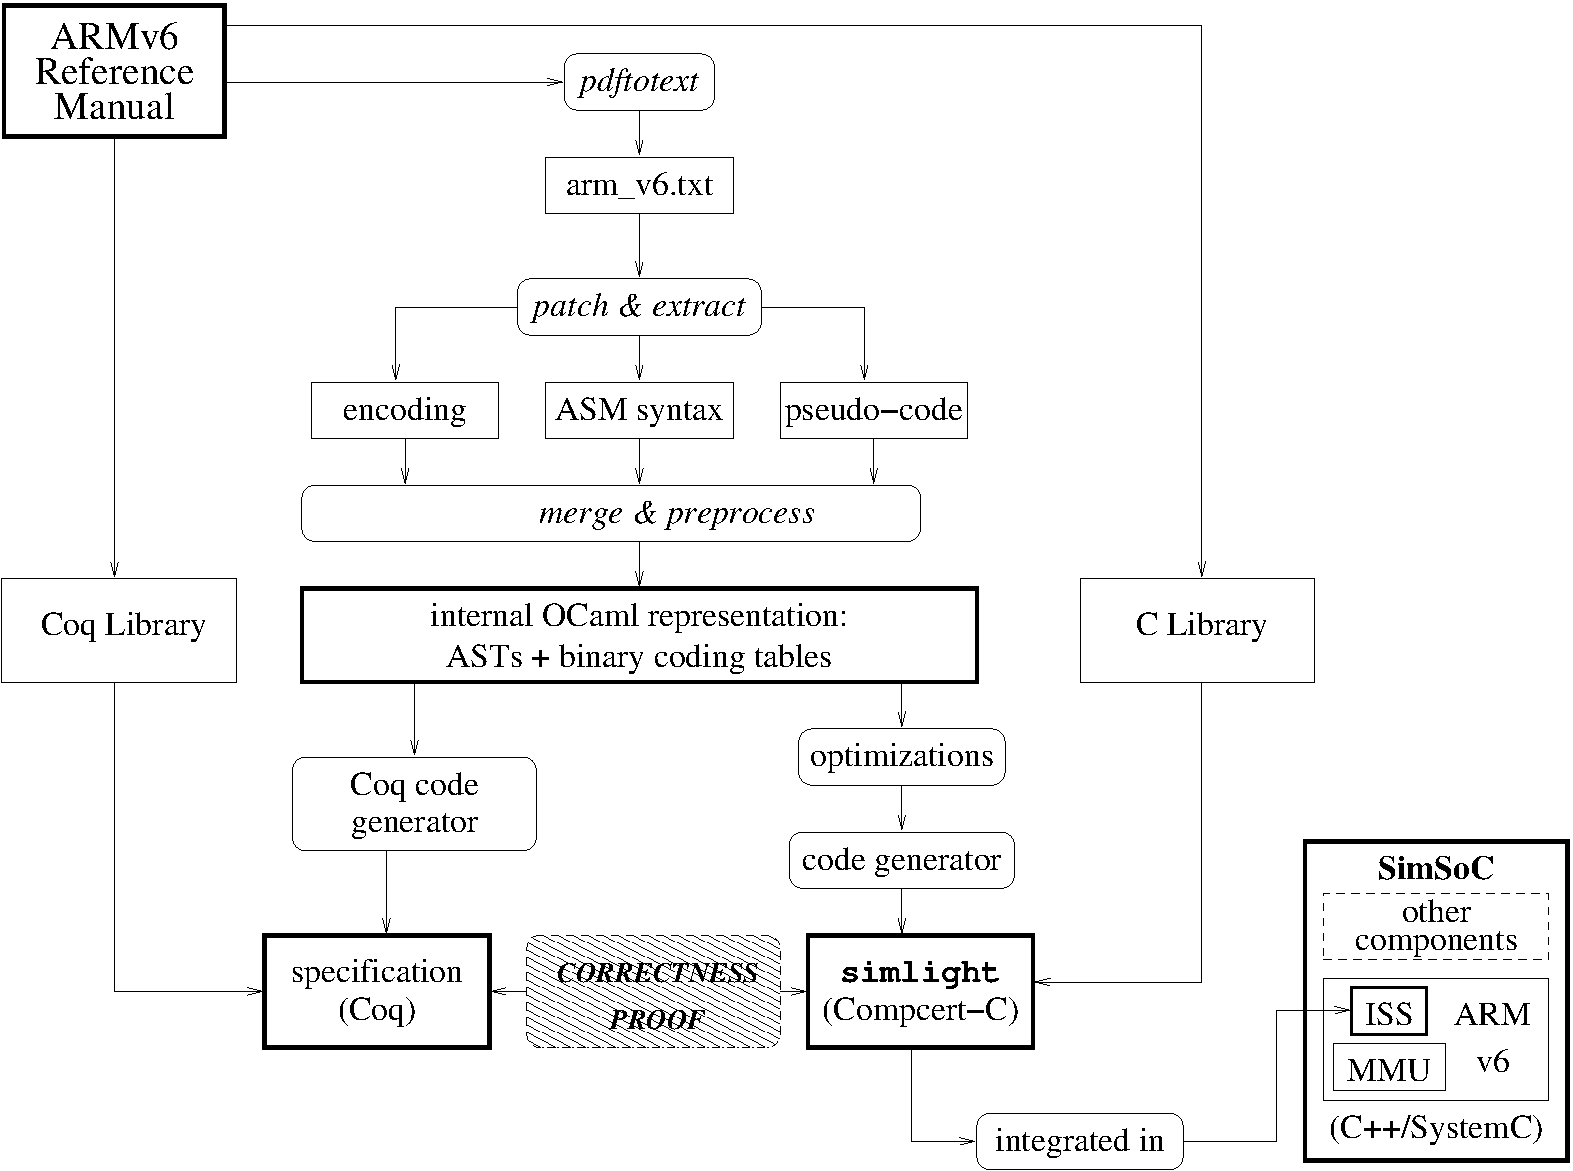
\includegraphics[width=\linewidth]{fig/fullarchi.pdf}
\caption{Overall generation chain}
\label{fig:arch}
\end{figure}

Three kinds of information are extracted for each ARM operation: its
binary encoding format, the corresponding assembly syntax, and its
body, which is an algorithm operating on various data structures
representing the state of an ARM: registers, memory, etc., according
to the fields of the operation considered. This algorithm may call
general purpose functions defined elsewhere in the manual, for which
we provide a \compcert C library to be used by the simulator and a Coq
library defining their semantics. The latter relies on libraries from
the \compcert project that allows us, for instance, to manipulate
32-bits representations of words. The result is a set of abstract
syntax trees (ASTs) and binary coding tables. These ASTs follow the
structure of the (not formally defined) pseudo-code.

In the end, two files are generated: a \compcert C file to be linked
with other components of \simsoc (each instruction can also be
executed in stand-alone mode, for test purposes for instance) and
files representing each instructions in \compcert C abstract syntax to
be used for correctness proof.

As the C language accepted by Compcert is a subset of the full ISO C
language, the generator has been constructed such that it only
generates C code in the subset accepted by the compcert compiler.
Nonetheless it can be compiled with other C compilers such as GCC
to obtain better performance. Even though in this case, the resulting
machine code is not guaranteed to be correct (there are well known
GCC optimization bugs...), at least the original C code has been
proven by our technique to be conformant with the ARM semantics.

The ARM V6 code generator not only generates the semantics functions,
it also generates the decoder of binary instructions supported in V6
architectures. This decoder is obtained by compiling the opcodes
information. The generated decoder is probably not optimal in
performance, but as \simsoc uses a cache to store the decoded
instructions, the performance penalty is marginal.

\subsection{Simulator Semantics}

In order to formally reason on the correctness of the simulator, we
need to have a formal model of the C implementation of the ARM
architecture generated as described above.  It is provided by \compcert,
which defines operational semantics of C formalized in Coq.

As the simulator C program also has the objective to achieve a high
speed simulator, the generator makes optimization. In particular,
states in the model of the C implementation are complex, not only due
to the inherent complexity of the C language memory model, but also
because of optimization and design decisions targeting efficiency.
In more detail:
\begin{itemize}
\item The C implementation uses large embedded \emph{struct}s to
  express the ARM processor state.  Consequently the model of the
  state is a complex Coq record type, including not only data fields
  but also proofs to guaranteed access permission, next block pointer,
  etc.
\item Transitions are defined with a relational style.  In general,
  the relational style is more flexible but functional definitions
  have some advantages: reasoning steps can be replaced by
  computations; existence and unicity of the result are automatically
  ensured.  However, the functional style is not always convenient or
  even possible.  It is the case here, where the transitions defined
  by the C implementation are relations which happen to be functions.
  This comes first from the operational semantics, which needs to be
  a relation for the sake of generality.  Furthermore in our case, the
  kind of record type mentioned in the previous item is too complex to
  execute calculation with it, so it is more convenient to describe
  the state transformation for memory with a relation.
\item The global state is based on a complex memory model with load
  and store functions that are used for read/write operations.
\end{itemize}

However, thanks to \compcert operational semantics, we are able to
formally express the semantics of the C implementation of the ARM
processor.

\subsection{Proof}

As a result of the generator described above, we have a C
implementation of the ARM instruction set.  To prove that it is
correct we need to have a formal specification of that architecture,
and prove that, given the initial state of the system, the execution
of an instruction as implemented by a C function results in the same
state as the formal specification.

Ideally the formal specification of the ARM architecture should be
provided by the vendor. But it is not the case, such a formal model is
not available on their web site, hence we had to build one.  As
mentioned in the related work section, we considered using the ARM
formal model defined in \cite{FoxM10}, but it would have required us
to translate all of the C operational semantics as well, which would
not have been error prone, not to mention the effort. So, we chose to
define a formal model of ARM architecture in Coq as well, derived from
the architecture reference manual. As Coq models are executable, we
could validate the model with real programs.

The state of the ARM V6 processor defined in the formal model is called
the \emph{abstract state}.  On the other hand, the same state is
represented by the data structures corresponding to C semantics that
we shall call the \emph{concrete state}.  In order to establish
correctness theorems we need to relate these two models.  Executing
the same instruction on the two sides produces a pair of new processor
states which should be related by the same correspondence. Informally,
executing the same instruction on a pair of equivalent states should
produce a new pair of equivalent states.

\begin{figure}
\hfil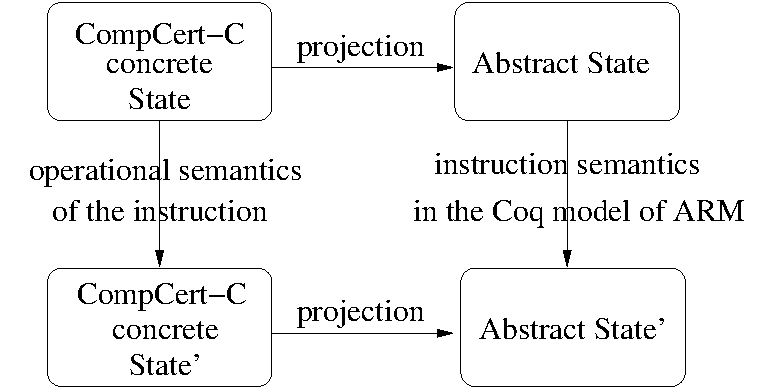
\includegraphics[width=.75\linewidth]{fig/theoremca.pdf}
\caption{Theorem statement for a given ARM instruction}
\label{fig:theoca}
\end{figure}

Our theorems arer schematized by Figure~\ref{fig:theoca}. The complete
proof is too lengthy for this article, and we only provide here an
outline of the method.  The correctness proof is based on one hand on
the semantics of the ARM architecture formal model, and on the other
hand on the \compcert C representation of the ARM instructions. We
need to prove that the operational semantics of that C code correspond
to the ARM formal specification.  The proof consists in defining
provable projections from the C state to the formal model to prove
their equivalence, as represented in Figure~\ref{fig:proj}.  To state
the correctness theorem, we compare the \compcert C semantics of a
function corresponding to an ARM instruction with its formal
definition.

For the C instruction set, we have a standalone C function for each
ARM V6 instruction.  Each function (instruction) has its own
correctness proof separately.  Every function is composed by its
return type, function parameters, local variables, and the function
body. The function body is a sequence of statements made of
expressions. Let us consider as an example the ARM instruction
\texttt{BL} (\texttt{Branch and Link}). The generated C code is:
\small{
\begin{verbatim}
void B(struct SLv6_Processor *proc,
       const bool L,
       const SLv6_Condition cond,
       const uint32_t signed_immed_24){
 if (ConditionPassed(&proc->cpsr, cond)){
  if ((L == 1))
   set_reg(proc,14,
           address_of_next_instruction(proc));
   set_pc_raw(proc,
         reg(proc,15)+
         (SignExtend_30(signed_immed_24)<<2));
 }
}
\end{verbatim}
}

The \compcert C representation of that C code is an internal
representation that can be externalized in a human readable form as:

\begin{alltt}\small
Definition fun_internal_B :=
\{|
 fn_return := void;
 fn_params := [
  proc -: `*` typ_SLv6_Processor;
  L -: int8;
  cond -: int32;
  signed_immed_24 -: uint32];
  fn_vars := [];
  fn_body :=\footnotesize
  `if (call (ConditionPassed`:T1)
        E[\&((`*(proc`:T2)`:T3)
         |cpsr`:T4)`:T5;cond`:T6] T7)
  then
   `if ((L`:T7)==(#1`:T6)`:T6)
      then (call (set_reg`:T8)
        E[proc`:T2; #14`:T6;
         (call (address_of_next_instruction`:T9)
                E[proc`:T2] T10)]
           T11)
   else skip;;
    (call (set_pc_raw`:T12)
      E[proc`:T2;
       (call (reg`:T13) E[proc`:T2; #15`:T6] T10)+
        ((call (SignExtend_30`:T14)
         E[signed_immed_24`:T10] T10)
           $<<$(#2`:T6)`:T10)`:T10]
      T11)
  else skip \small
 |\}.
\end{alltt}

The main strategy is to define a projection from the concrete state to
the abstract state.  On both sides, the execution of an instruction is
described by a state transition.  For the two representations,
``State'' refers to the full description of the system. This
correspondance is expressed by a projection relating the two models of
the state.

\begin{figure}[h]
\hfil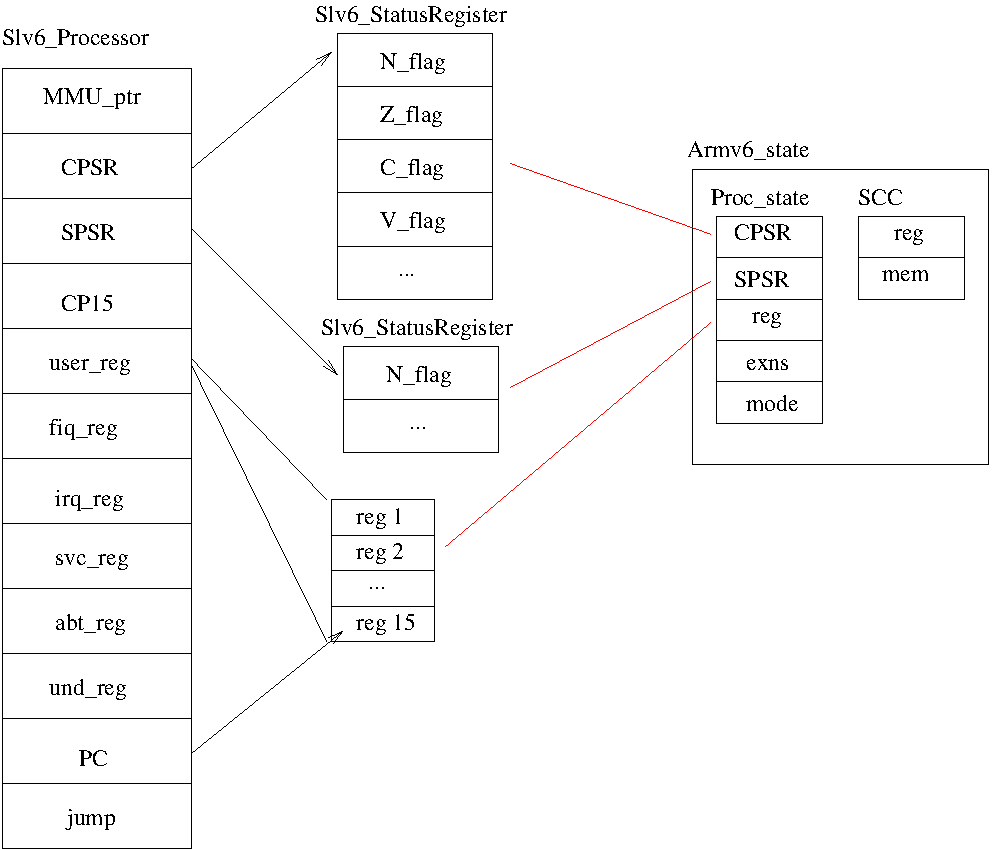
\includegraphics[width=.75\linewidth]{fig/projection.pdf}
\caption{Projection}
\label{fig:proj}
\end{figure}
According to the type of the argument of the projection, the
definitions of projections are different.  For example, the projection
of a register performs a case analysis on a value of type
\texttt{register}, whereas the projection of SPSR (Save Processor
Status Register) depends on the type of exception modes.  We define a
specific projection for each type.  Although Coq is rich enough to
allow for the definition of a general projection for all types of
elements, using dependent types, we chose to define a projection
relation for each instance to improve readability of the proofs.
The proofs start from the abstract state described by the formal
specification.  An issue is that C representations introduce a complex
memory model designed for high simulation speed, and we need a mapping
to the formal model. In order to verify the projection of the pair of
original states, we need the following data: the initial memory state,
the local environment, and the formal initial processor state.  The
projection is meaningful only after the C memory state is prepared for
evaluating the current function body representing a ARM instruction.
In the abstract Coq model, we directly use the processor state
\texttt{st}.  But on the C side, the memory state must provide the
contents of every parameter, especially the memory representation of
the processor state.  We also need to observe the modification of
certain blocks of memory corresponding to local variables.

Fortunately \compcert formalizes the C memory model.  The semantics of
\compcert C consider two environments. The global environment
\emph{genv} maps global function identifiers, global variables
identifiers to their blocks in memory, and function pointers to a
function definition body.  The local environment \emph{env} maps local
variables of a function to their memory blocks reference.  It maps
each variable identifier to its location and its type, and its value
is stored in the associated memory block.  The value associated to a C
variable or a parameter of a C function is obtained by applying
(abstract) \texttt{load} to the suitable reference block in memory.
These two operations are performed when a function is called, building
a local environment and an initialized memory state. When the program
starts its execution, \emph{genv} is built.  On the other hand,
\emph{env} is built when the associated function starts to allocate
its variables. Therefore, on \compcert C side, a memory state and a
local environment is prepared initially using two steps. First,
allocate function variables: from an empty local environment, all
function parameters and local variables ara allocated into the memory
state, yielding a new memory state and the local environment. Second,
initialize function parameters: using a function
\texttt{bind\_parameters} to initialize parameters with a list of
argument values and a new memory state is created.

Now we have all elements ready to make the projection from the local
environment to the abstract state to verify their equivalence.
Next, we need to consider the execution of the instruction.  \compcert
has designed semantics for \compcert C in both small-step and
big-step.  The big-step inductive type for evaluating expression is
enough for our proof.  The semantics is defined as a relation between
an initial expression and an output expression after evaluation.  Then
the body of the function is executed.  On the \compcert C side, the
execution is yielding a new memory state \textbf{mfin}.  On the
abstract side, the new processor state is obtained by running the
formal model.  Finally, we have to verify that the projection from the
concrete state \textbf{mfin} should provide the latter abstract
state.  Note that all projections are performed using the same local
environment \texttt{e}.

The formal model of ARM V6 is defined as a much simpler functional
model and computing the value of a component can be performed
directly.

The proof is performed in a top-down manner. It follows the definition
of the instruction, analyzing the expression step by step.  The
function body is split into statements and then into expressions.
When evaluating an expression, we search for two kinds of information.
the first one is how the memory state changes on \compcert C side; the other is
whether the results on the abstract and the concrete model are related
by the projection. To this effect, we use mostly the following lemmas.

\begin{enumerate}
\item
  \textit{Lemma: Evaluating a \compcert expression with no modification on the memory state.}\\
  This lemma is concerned with the expression evaluation on \compcert
  C side and in particular the C memory state change issue.  Asserting
  that a memory state is not modified has two aspects: one is that the
  memory contents are not modified; the other is that the memory
  access permission is not changed.  For example, evaluating the
  boolean expression $Sbit~==~1$ returns an unchanged memory state.
\begin{align*}
%&
\textrm{if}~~ G,E~\vdash \texttt{eval\_binop}_c~(Sbit~==~1),\\
\:M~\xLongrightarrow{\varepsilon}~vres,\:M'
%&
\textrm{then}~~ M=M'.
\end{align*}
In Coq syntax, the relation in premise is expressed with
\texttt{eval\_binop}, a companion predicate of \texttt{exec\_stmt}
above, devoted to binary operations.  In this lemma and the following,
$E$ is the local environment, $G$ is the global environment and $M$ is
the memory state; $\varepsilon$ is the empty event (\texttt{Events.E0}
in Coq syntax); usually $t$ is used to represent a series of system
events; $vres$ is the result.  Here, $vres$ is not important.  The
evaluation is performed under environments $G$ and $E$.  Before
evaluation, we are in memory state $M$.  With no event occurring, we
get the next memory state $M'$. According to the definition of
\texttt{eval\_binop}, an internal memory state will be introduced.
\begin{center}
$\dfrac
{G,E~\vdash a_1,M\Rightarrow M'~~~G,E~\vdash a_2,M'\Rightarrow M''
}
{G,E~\vdash (a_1~binop~a_2),M\Rightarrow~M''}$
\end{center}

Now, in our example, expression $a_1$ is the value of $Sbit$ and $a_2$
is the constant value $1$.  By inverting the hypothesis of type
\texttt{eval\_binop}, we obtain several new hypotheses, including on
the evaluation of the two subexpressions and the introduction of an
intermediate memory state $M''$.  Evaluating them has no change on the
C memory state.  Then we have $M = M'' = M'$.  In more detail, from
the \compcert C semantics definition, we know that, evaluation of an
expression will change the memory state if the evaluation contains
uses of \texttt{store\_value\_of\_type} (in \compcert versions before
1.11), which stores the value in memory at a given block reference and
memory chunk.  In \compcert-1.11, the basic store function on memory
is represented by an inductive type \texttt{assign\_loc} instead of
\texttt{store\_value\_of\_type}.  Since \compcert version 1.11
introduced volatile memory access, we have to determine whether the
object type is volatile before storage, and also type size in addition
of the access mode.
\item
\textit{Lemma: Result of the evaluation of an expression with no modification on the memory.}
Continuing the example above, we now discuss the result of evaluating
the binary operation $Sbit~==~1$ both in the abstract and the concrete model.
At the end of evaluation, a boolean value $true$ or $false$ should be returned.
in both the \compcert C model and the formal model,
using the projection definition.
\begin{align*}
\textrm{if} ~ \texttt{Sbit\_related}~M~\texttt{Sbit},\\
\textrm{and} ~ G,E~\vdash \texttt{eval\_rvalue\_binop}_c~(Sbit~==~1),\\
M\Rightarrow~v,\textrm{then} ~ v=(Sbit~==~1)_{coq}
\end{align*}
Intuitively, if the projection corresponding to the parameter
\texttt{sbit} in the C program yields the right information from the
abstract state, then the evaluation will return the same value both in
the abstract and in the concrete model.  Here, the expression is a
so-called ``simple expression'' that always terminates in a
deterministic way, and preserves the memory state.
To evaluate the value of simple expressions, \compcert provides two
other big-step relations \texttt{eval\_simple\_rvalue} and
\texttt{eval\_simple\_lvalue} for evaluating respectively their left
and right values.  The rules have the following shape:
\[
\dfrac{
\begin{array}{l}
G,E~\vdash a_1,M\Rightarrow v_1 \quad G,E~\vdash a_2,M\Rightarrow v_2\\
\texttt{sem\_binary\_operation}(op,v_1,v_2,M)~=~v
\end{array}}
{G,E~\vdash (a_1~op~a_2),M\Rightarrow v}
\]
In order to evaluate the binary expression $a_1~op~a_2$,
the sub-expressions $a_1$ and $a_2$ are first evaluated,
and their respective results $v_1$ and $v_2$ are used
to compute the final result $v$.
\item
  {\it Lemma : Memory state changed by storage operation or side effects of evaluating expression}\\
  As mentioned before, evaluating some expressions such as
  \texttt{eval\_assign} can modify the memory state.  Then we need
  lemmas stating that corresponding variables in the abstract and in
  the concrete model will evolve consistently.  For example, this is
  stated as follows for an assignment on register $Rn$.  Here we use
  the projection relation \texttt{register\_related}. Expressions with
  side effects of modifying memory are very similar.
\begin{align*}
&\textrm{if} ~~ \texttt{rn\_related}~M~rn\\
&\textrm{and}~~  G,E~\vdash \texttt{eval\_assign}_c~(rn:=rx),M~\Rightarrow~ M',v\\
&\textrm{then} ~~ \texttt{rn\_related}~M'~rn
\end{align*}
\item
  \textit{Lemma: Internal function call.}\\
  Internal functions are described in an informal manner in the ARM V6
  reference manual.  No pseudo-code is available for them, which means
  that the corresponding library functions, both in the abstract model
  and in C, are coded manually.  In order to get a suitable
  \compcert C AST to reason about, we use the parser provided in
  \compcert.  When combining the simulation code of an instruction
  with the code of library functions, we need to take care of the
  memory allocation problem.  In \compcert C representation,
  identifiers are unique positive numbers which indicate the memory
  block where corresponding variables are allocated.  Currently, the
  extra identifiers introduced by library functions are added manually
  and assigned with fresh block numbers.
\label{page:libfunast}
\begin{align*}
&\textrm{if} ~~  \texttt{proc\_state\_related}~M~st \\
&\textrm{and} ~~ G,E~\vdash \texttt{eval\_funcall}_c\\
&        (copy\_StatusRegister)_c,M\Rightarrow~v,~M'\\
&\textrm{and} ~~ st'~=~(copy\_StatusRegister)_{coq}~st\\
&\textrm{then} ~~\texttt{proc\_state\_related}~M'~st'.
\end{align*}
After an internal function is called, a new stack of blocks is
allocated in memory.  After the evaluation of the function is
performed, these blocks will be freed.  Unfortunately, this may not
bring the memory back to the previous state: the memory contents may
stay the same, but the pointers and memory organization may have
changed. For lemmas on evaluation of internal functions, we can
observe the returned result on variables, compare it with the
corresponding evaluation in the formal specification, and verify some
conditions.  For example, the lemma above is about the processor state
after evaluating an internal function call
\texttt{copy\_StatusRegister} which reads the value of CPSR and then
assigns it to SPSR.  The evaluation of \texttt{copy\_StatusRegister}
should be protected by a check on the current processor mode.  If it
is neither system mode nor user mode, the function
\texttt{copy\_StatusRegister} can be called.  Otherwise, the result is
``unpredictable'', which is defined by ARM architecture

It is then necessary to reason on the newly returned states, which
should still be related by the projection.  This step is usually easy
to prove, by calculation on the two representations of the processor
state to verify they match.
\item 
\textit{Lemma: External function call.}\\
The \compcert C AST of an external function call contains the types of
input arguments and of the returned value, and an empty body.
\compcert provides the expected properties of a few built-in external
functions such as \texttt{printf}, \texttt{malloc} and \texttt{free}.
We have proceeded similarly for the external functions of the ARM
simulator.  The general expected properties of an external call are
that (i) the call returns an result, which has to be related to the
abstract state, (ii) the number of arguments must agree with the
signature.  (iii) after the call, no memory blocks are invalidated,
(iv) the call does not increase the access permission of any valid
block, and finally that the memory state can be modified only when the
access permission of the call is maximal. For each external call, we
verify the required properties.
\end{enumerate}

In addition to the above lemmas we had to prove a fair number of more
trivial lemmas that are omitted here.  Most of them are related to the
semantics of \compcert C.  With these lemmas we can build the proof
scripts for ARM instructions.  For that, we are decomposing the ARM
instruction execution step by step to perform the execution of
the C programs . \compcert C operational semantics define large and
complex inductive relations. Each constructor describes the
memory state transformation of an expression, statement, or function.
As soon as we want to discover the relation between memory states
before and after evaluating the C code, we have to invert the
hypotheses of operational semantics to follow the clue given by its
definition, to verify the hypotheses relating concrete memory states
according to the operational semantics.

During the development of a proof, if a hypothesis is an instance of
an inductive predicate and we want to derive the consequences of this
hypothesis, the general logical principle to be used is called
\emph{inversion}. An {\em inversion} is a kind of forward reasoning
step that allows for users to extract all useful information contained
in a hypothesis.  It is an analysis over the given hypothesis according
to its specific arguments, that removes absurd cases, introduces
relevant premises in the environment and performs suitable
substitutions in the whole goal.  The practical need for automating
inversion has been identified many years ago and most proof assistants
(Isabelle, Coq, Matita,...)  provide an inversion mechanism.  To this
effect, the Coq proof assistant provides a useful tactic called
\inversion \cite{coqmanual}.
% which is available in several variants, including the {\em small inversion}~\cite{small-inversion}.

Every instruction contains complex expressions, but each use of
\inversion will go one step only.  If we want to find the relation
between the memory states affected by these expressions, we have to
invert many times. For illustration, let us consider the simple
example from the ARM reference manual \texttt{CPSR = SPSR}.  As
the status register is not implemented by a single value, but a set of
individual fields, the corresponding C code is a call to the function
\texttt{copy\_StatusRegister}, which sets the CPSR field by field with
the values from SPSR.  Lemma \texttt{same\_cp\_SR} below states that
the C memory state of the simulator and the corresponding formal
representation of ARM processor state evolve consistently during this
assignment.
\begin{alltt}\small
Lemma same_copy_SR :
  forall e m l b s t m' v em,
  proc_state_related m e
   (Ok tt (mk_semstate l b s)) ->
      eval_expression
       (Genv.globalenv prog_adc)
          e m expr_cp_SR t m' v ->
          forall l b,
          proc_state_related m' e
          (Ok tt
           (mk_semstate l b
             (Arm6_State.set_cpsr s
             (Arm6_State.spsr s em))))
\end{alltt}
From this, we have to invert generated hypotheses until all
constructors used in its type are exhausted. On this example, 18
consecutive inversions are needed... The first proofs scripts we wrote
were becoming unmanageable, and not robust to version changes of Coq
or \compcert.  In order to reduce the script size and get better
maintainability, we studied a general solution to this problem, and
developed a new inversion tactic in Coq. % \cite{small-inversion,itp13}. 
We have first expanded 
small inversion mechanism from previous work and added a new inversion tactic
for inductive types in \compcert.  The semantics of \compcert C tells
us how the memory state is transformed by evaluating expressions.
Using the built-in constructs of the tactics language, we can define a
high-level tactic for each inductive type, gathering all the functions
defined for its constructors.

This tactic has two arguments corresponding to the C memory states.
The first step of the tactics introduces generated components with new
names.  The second step is related to previously reverted hypotheses,
ensuring that the new names introduced are correctly managed by Coq.
The tactic then proceeds as follows. First, it automatically finds the
hypothesis to invert by matching the targeted memory states
and the related hypotheses are reverted; next the right auxiliary
function is called (all auxiliary functions are gathered in the
tactic) and meaningful names are given to derived variables and
hypotheses, next all other related hypotheses are updated according to the new names
and new values and useless variables and hypotheses are cleaned up.
Finally the steps above are repeated until all transitions between
the two targeted memory states are discovered.
\noindent
As a result, considering the former example of \texttt{same\_copy\_SR}
where 18 standard \inv were used in the first proof script we
developed, our tactics reduced them in one step:
\texttt{inv\_eval\_expr~m~m'}.  Thanks to this new tactics, the size
of the proofs has become smaller and the proof scripts are more
manageable. The size vary with the instructions complexity from less
than 200 lines (e.g 170 for LDRB) to over 1000 (1204 for ADC).  As a
result, for each ARM instruction, we have established a theorem
proving that the C code simulating an ARM instruction is equivalent to
the formal specification of the ARM processor. All of these lemmas and
theorems are verified by the Coq theorem prover.

\section{Certified Simulation}

Based on the work afore mentioned, we can now consider the certified
execution of a C program. We take here as an example the DES
cryptographic encryption code.  The C code for encrypting a block of
data is straightforward:
\small{\begin{verbatim}
#define GET_ULONG_BE(n,b,i)
 (n)=((unsigned long)(b)[(i)]<<24)
    |((unsigned long)(b)[(i)+1]<<16)
    |((unsigned long)(b)[(i)+2]<<8)
    |((unsigned long)(b)[(i)+3] );

#define DES_IP(X,Y)
    T =((X>>4)^Y)&0x0F0F0F0F;
    Y^=T;X^=(T<<4);
    T=((X>>16)^Y)&0x0000FFFF;
    Y^=T;X^=(T<<16);
    T=((Y>>2)^X)&0x33333333;
    X^=T;Y^=(T<<2);
    T=((Y>>8)^X)&0x00FF00FF;
    X^=T;Y^=(T<<8);
    Y=((Y<<1)|(Y>>31))&0xFFFFFFFF;
    T=(X^Y)&0xAAAAAAAA;
    Y ^=T;X^= T;
   X=((X<<1)|(X>>31))&0xFFFFFFFF;

#define DES_ROUND(X,Y)
    T=*key++^X;
    Y^=SB8[(T)&0x3F]
       ^SB6[(T>>8)&0x3F]
       ^SB4[(T>>16)&0x3F]
       ^SB2[(T>>24)&0x3F];
    T=*key++^((X<<28)|(X>>4));
    Y^=SB7[(T)&0x3F]
       ^SB5[(T>>8)&0x3F]
       ^SB3[(T>>16)&0x3F]
       ^SB1[(T>>24)&0x3F];

void des_crypt_ecb(unsigned long *key,
               unsigned char input[8],
             unsigned char output[8] ){
    int i;
    unsigned long X,Y,T;
    GET_ULONG_BE(X,input,0);
    GET_ULONG_BE(Y,input,4);
    DES_IP(X,Y);
    for(i=0;i<8;i++) {
        DES_ROUND(Y,X);
        DES_ROUND(X,Y);
    }
    DES_FP(Y,X);
    PUT_ULONG_BE(Y,output,0);
    PUT_ULONG_BE(X,output,4);
}
\end{verbatim}
}

Looking at the binary code of that function generated by the compiler,
one may observe that this code actually uses only 22 different types of ARM
instructions, namely \textbf{ add, and, asr, b, ble, bne, bx, cmp,
  eor, ldm, ldr, ldrb, lsl, lsr, mov, orr, pop, push, str, str, strb,
  sub}.

Given that we have a proof that the machine code generated from C is
correct, thanks to \compcert, and now a proof of the ARM instruction
set for these instructions, we have a proof that the simulation of the
DES algorithm on our ARM simulator is conformant with the algorithm.


%%%%%%%%%%%%%%%%%%%%%%%%%%%%%%%%%%%%%%%%%%%%%%%%%%%%%%%%%%%%%%%%%
\section{Conclusion}
\label{conclusion}
We have constructed a tool chain that makes it possible to certify
that the simulation of a program is conformant with the formal
definition of the algorithm, by leveraging off from three existing
tools namely, Compcert-C, that has defined formal C semantics and a
formally proven the code generator, Coq and SimSoc, to which we have
added a proven generated simulator of the ARM instruction set.

Although we have considered a small example in the paper, there is no
limit on the size of the C code that can be certified as long as
the instruction set has been certified.

In fact, if there existed a publicly availale formal model of the ARM
processor approved by ARM Ltd company, our work could be construed
to define a certified execution of a C program.

We acknowledge a weak point in our chain, due to the fact that the
hardware vendors do not provide formal semantics of their instruction
set. Because such formal models are unavailable, we had to define a
formal model of ARM processor ourselves, which may be wrong.  As Coq
specifications are executable, we have been able to validate our ARM
formal model by checking that we obtain identical results with real
test programs, but this is not a formal proof... If the vendors would
make public formal specifications of their architectures, then our
toolchain could become fully verified.

Finally, assuming that the real ARM chips commercialized by the
various circuit vendors are indeed implementations of our formal
model, an outcome of our work is that, since we prove the execution of
programs over a simulator that is itself a proved implementation of
the architecture, it means then that the execution of programs that
are themselves generated from formal specifications (C programs
generated from formal models with a certified generator) on that
architecture are proved to be correct with regards to their
specification. This assumption remains to be proved but we believe
however that it represents a significant step forward.


%%%%%%%%%%%%%%%%%%%%%%%%%%%%%%%%%%%%%%%%%%%%%%%%%%%%%%%%%%%%%%%%%%
\section*{Acknowledgments}

Removed for review.
% This work has been supported jointly by INRIA, Tsinghua University,
% Shenzhen Institutes of Advanced Technology, Chinese Academy of
% Sciences.

%%%%%%%%%%%%%%%%%%%%%%%%%%%%%%%%%%%%%%%%%%%%%%%%%%%%%%%%%%%%%%%%%%


\bibliographystyle{plain}
\bibliography{references}


\end{document}
